\chapter{Software}
\label{chap:software}
%
% preface chapter
\lettrine[lines=3]{T}{his} chapter describes the software developed for the
hardware described in the chapter. The choice to use the Qt framework guarantees
the portability of the code thanks to the cross-platform support. The software
is divided into two programs capable of communicating with each other: the first
works on Raspberry Pi and allows the user to interface easily with the FLir
thermal camera and with the Raspicam camera. It also acts as a TCP server for
sending the images shot to connected devices. The second part is a client
program that receives the data sent by the main device, and allows the analysis
of the image through machine learning on dedicated hardware.
%
% input files
%
% introduction
\section{Interface}
\label{sec:raspberry-software}
As anticipated, the software run on the Raspberry Pi is made following the
paradigm of object-oriented programming. Made in C ++\/Qt making extensive use
of the proprietary classes of the framework and the Standard Template Library
(STL). This program has some dependencies with regard to the thermal camera
drivers supplied by the manufacturer and are 32-bit, since the Raspberry Pi 3,
described in \ref{sec:raspi3}, is equipped with a 32-bit ARM Cortex-A53
processor. These allow total control of the camera. The second dependency is the
Raspicam library which allows the interface with the RGB camera allowing the
image acquisition.
%
\begin{figure}[htb]
	\centering
	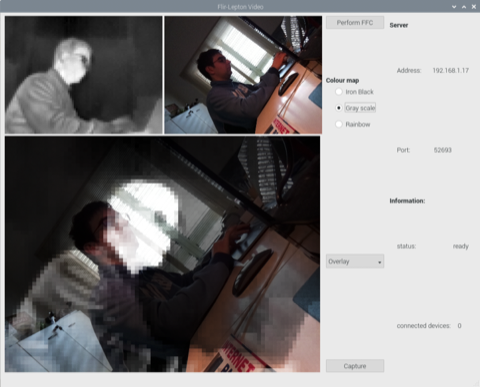
\includegraphics[width=0.65\textwidth]{grayscale.png}
	\caption{User interface run on Raspberry Pi 3b.}
	\label{fig:software-main-ui}
\end{figure}
%
% interface
Continuing a user interface has been created through the use of widgets, this is
divided into three areas. The first area shows the video streams acquired
separately in two labels, the third larger label shows the two streams mixed
through filters made available as default the overlay filter is used. It was
preferred not to perform a match of the images with pixel-by-pixel recalculation
for two reasons: the first due to the high difference in size of the sensors as
that of the thermal camera is $80 \times 60$ pixels while the raspicam is $3280
\times 2464$ pixels. The second is to not aggravate the computational load on
the CPU. The second area provides some controls for the user, in fact it is
possible to save thermal images on files during the acquisition. you can change
the heat map applied to the image on the fly by choosing from three different
possibilities, in the figure you can observe the result. 
Finally, it is possible to modify the mixing filter, also on the fly, of the
video streams to obtain different effects to improve visibility or to increase
details. The last section of the user interface shows the information relating
to the TCP socket used for sending the video stream to other devices.
%
% image ui
\begin{figure}[htb]
    \centering
    \subfloat[][\emph{lava}.\label{subfig:lava-map}]
        {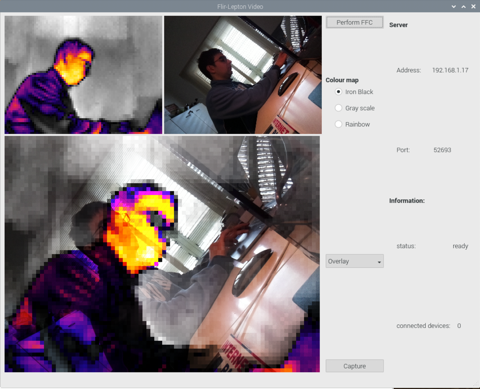
\includegraphics[width=.30\textwidth]{lava.png}} \quad
    \subfloat[][\emph{grayscale}.\label{subfig:grayscale-map}]
        {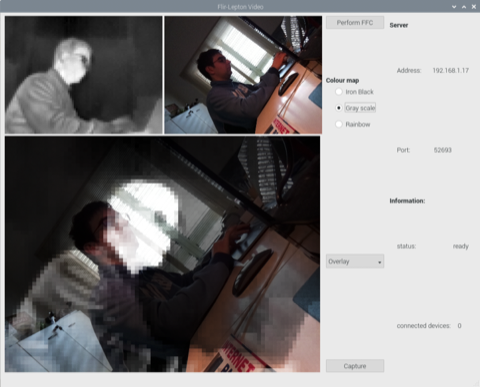
\includegraphics[width=.30\textwidth]{grayscale.png}} \quad
    \subfloat[][\emph{rainbow}.\label{subfig:rainbow-map}]
        {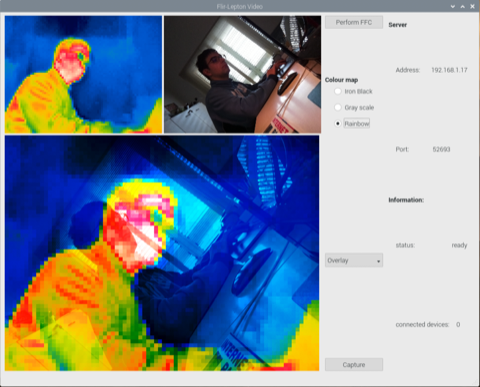
\includegraphics[width=.30\textwidth]{rainbow.png}}
    \caption{Result colourization applied to thermal camera data.}
    \label{fig:reuslt-maps}
\end{figure}
%
% software analysis 
\subsection{Software Analysis}
\label{ssec:raspberry-softw-analysis}
The user interface is run on the main thread, in order to maximize the
performance of the executed code the image acquisition operation is performed in
the secondary thread. Thanks to the use of the signal and slot system of Qt it
is possible to update the labels without blocks typical of multi-threaded
programming. 
The difficulty of concurrent programming usually consists in
synchronizing the access to resources by different threads that act in
competition on the same resources. Having two or more threads accessing the same
data simultaneously can lead to unexpected and unwanted results. 
In fact, without the application of particular programming techniques, it is not
possible to predict in a deterministic way, at the time of execution, when that
specific thread will be executed: their progression depends on the priorities
decided by the scheduler of the operating system and not by the programmer. 
In fact, multiple threads can access the same variable and modify its content or
value. Therefore, synchronization techniques such as mutual exclusion are used
to solve the problem. As a result, ideally a thread should execute code as
independent of the rest of the program as possible. Furthermore, errors in
synchronization between threads are often very difficult to detect because their
occurrence essentially depends on the environment in which the program is run.
The synchronization of one thread with another is normally necessary to allow
them to communicate with each other and to return the results of a function to
the main process; it is normally done through \emph{mutex}\cite{wiki:thread}.
Analysing the code of the thread that takes care of acquiring the images we can 
see that it proceeds without mutex\footnote{The mutex class is a synchronization
primitive that can be used to protect shared data from being simultaneously
accessed by multiple threads.}, but uses the signal and slot system as mentioned
before.
%
% code list
\begin{listing}[ht] 
\inputminted[bgcolor=bg,frame=lines,framesep=2mm, linenos=true, autogobble, breaklines=true, fontsize=\scriptsize]{c++}{software/code/leptonthread.cpp} 
\caption{Infinite loop thread cameras.} 
\label{lst:leptonthread} 
\end{listing}
%




















\section{Introduction}
\label{sec:intro}
In this era, a large amount of structured and unstructured data became
available. \textbf{Machine Learning} (\textbf{ML}) has evolved as a branch of
artificial intelligence: it envisages the development of self-learning
algorithms, which are capable of acquiring knowledge from data with the aim of
making predictions. Instead of requiring a human presence who manually enact the
rules and build models for the analysis of large amounts of data, machine
learning offers a more efficient alternative to capture the knowledge in the
data. Machine learning aims to gradually improve the performance of forecasting
models and to make data driven decisions. In this section we will examine the
three different types of machine learning: \emph{supervised learning},
\emph{unsupervised learning} and \emph{reinforcement learning}. Where we will
show the fundamental differences between these types of
learning.\cite{raschka2016machine}
%
\subsection{Supervised learning}
\label{subsec:supervised-learnig}
The main purpose of supervised learning is to derive a model from  training
data, which allows us to make predictions for data that are not available or
future. Here, the term ``supervision" refers to the fact that the output signal
labels  of the sample sets are already known. A supervised learning task, which
is based on discrete class labels, is also  called a classification task, in
figure \ref{fig:supervised-learning-scheme} it  is possible to observe a process
diagram. Another supervised learning subcategory is regression, whose resulting
signal is a continuous value. Classification is a sub-category of supervised
learning, which has the goal to provide class category labels for new instances,
based on observations made in the past.

These labels are discrete, unordered values that can be considered as belonging
to a group of instances. However, the set of class labels does not necessarily
have to be a binary nature. The predictive model identified by a supervised
learning algorithm can consider each class label that is present in the learning
dataset of a new instance, which is not labelled. A typical example of
\emph{multi-class classification} is the recognition of hand-written
text.\cite{raschka2016machine}
%
\begin{figure}[!h]
\centering
%\draw [help lines] (0,0) grid (8,8);
\resizebox{0.65\textwidth}{!}{\begin{tikzpicture}[auto,>=latex']
%\draw [help lines] (0,0) grid (8,8);
\tikzset{
	boxA/.style={
  		rectangle,
  		inner sep=0pt,
  		text width=25mm,
  		align=center,
  		draw=black,
  		fill=airforceblue,
  		minimum height = 10mm
  	},
  	boxB/.style={
  		rectangle,
  		inner sep=0pt,
  		text width=25mm,
  		align=center,
  		draw=black,
  		fill=amber,
  		minimum height = 10mm
  	},
  	boxB1/.style={
  		rectangle,
  		inner sep=0pt,
  		text width=25mm,
  		align=center,
  		draw=black,
  		fill=amber!30,
  		minimum height = 10mm
  	},
  	boxC/.style={
  		rectangle,
  		inner sep=0pt,
  		text width=25mm,
  		align=center,
  		draw=black,
  		fill=light-gray,
  		minimum height = 10mm
  	},
  }

\node (a) [boxC, align=center] at (1,1) {New data};
\node (b) [boxC, align=center] at (5,1) {Predicitve\\ model};
\node (c) [boxC, align=center] at (9,1) {Prediction};
\node (d) [boxA, align=center] at (5,3) {Alogrithm\\ DNN};
\node (e) [boxB, align=center] at (5,5) {Dataset};
\node (e1) [boxB1, align=center] at (6,5.85) {Label};
\draw [->] (a) -- (b);
\draw [->] (b) -- (c);
\draw [->] (d) -- (b); 
\draw [->] (e) -- (d); 
\end{tikzpicture}}
\caption{supervised learning scheme} 
\label{fig:supervised-learning-scheme}
\end{figure}
%
\subsection{Reinforcement learnig}
\label{subsec:reinforcement-learnig}
Another type of machine learning is reinforcement learning. Here, the goal is to
develop a system (\emph{agent}) for people to improve their performance. In
order to do so, that system is based on interactions with  the environment.
Since information relating to the current state of the environment include also
a \emph{reward} signal, we can consider strengthening learning as an example of
supervised learning. However, this feedback is not the correct label or the true
value of truth, but it represents the quality of the measurement of the 
performance measured by the reward function. Through interaction with the
environment, an agent can then use reinforcement learning to learn a series of
actions, which maximize this reward through a trial-and-error exploratory
approach or deliberative planning.\cite{raschka2016machine}
%
\begin{figure}[!h]
\centering
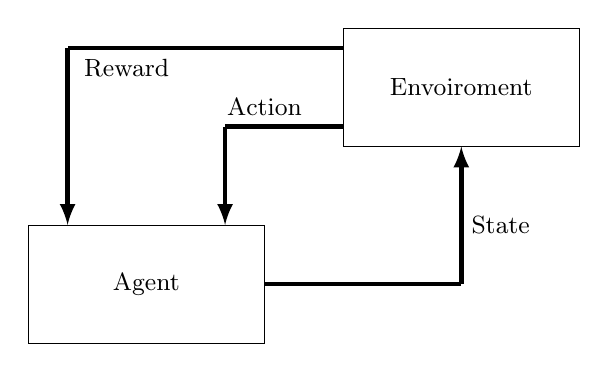
\begin{tikzpicture}[>=latex]
 %\draw [help lines] (0,0) grid [step=0.5] (8,4);
 \draw (0.5,0) rectangle ++(3cm, 1.5cm);
 \draw (4.5,2.5) rectangle ++(3cm,1.5cm);
 %\node [draw] (1.5,2) {Agent};
 \coordinate [label={[font=\small]center:Agent}] (A) at (2,0.75);
 \coordinate [label={[font=\small]center:Envoiroment}] (E) at (6,3.25);
 \draw [-, ultra thick] (3.5,0.75) -- (6,0.75);
 \draw [->, ultra thick] (6,.75) -- (6,2.5);
 \coordinate [label={[font=\small]center:State}] (S) at (6.5,1.5);
 %
 \draw [-, ultra thick] (4.5,2.75) -- (3,2.75);
 \draw [->, ultra thick] (3,2.75) -- (3,1.5);
 \coordinate [label={[font=\small]center:Action}] (T) at (3.5,3);
 %
 \draw [-, ultra thick] (4.5,3.75) -- (1,3.75);
 \draw [->, ultra thick] (1,3.75) -- (1,1.5);
 \coordinate [label={[font=\small]center:Reward}] (R) at (1.75,3.5);
\end{tikzpicture} 
\caption{reinforcement learning scheme} 
\label{fig:reinforcement-learning-scheme}
\end{figure}
%
\subsection{Unsupervised learning}
\label{subsec:unsupervised-learning}
In supervised learning, we know in advance the correct answer when we describe
our model, while in reinforcement learning we define a measure, or reward, for
the specific actions performed by the agent. In unsupervised learning, on the
other hand, we are dealing with unlabelled data or data from the unknown
structure. Using unsupervised learning techniques, we are able to observe the
structure of our data, to extract meaningful information from them without being
able to rely on the guide nor a variable known relative result, nor a reward
function. Clustering is an exploratory technique of data analysis that allows us
to organize a series of information within meaningful groups (\emph{cluster})
without having any previous knowledge of memberships in such groups. Each
cluster that can be derived during the analysis defines a group of objects that
share a certain degree of similarity, but which are more dissimilar than the
objects present in the other clusters, which is why clustering is sometimes
called \emph{``unsupervised classification"}. Clustering is an excellent
technique for structuring information to identify meaningful relationships in
the data.\cite{raschka2016machine}
%
\begin{figure}[!h]
\centering
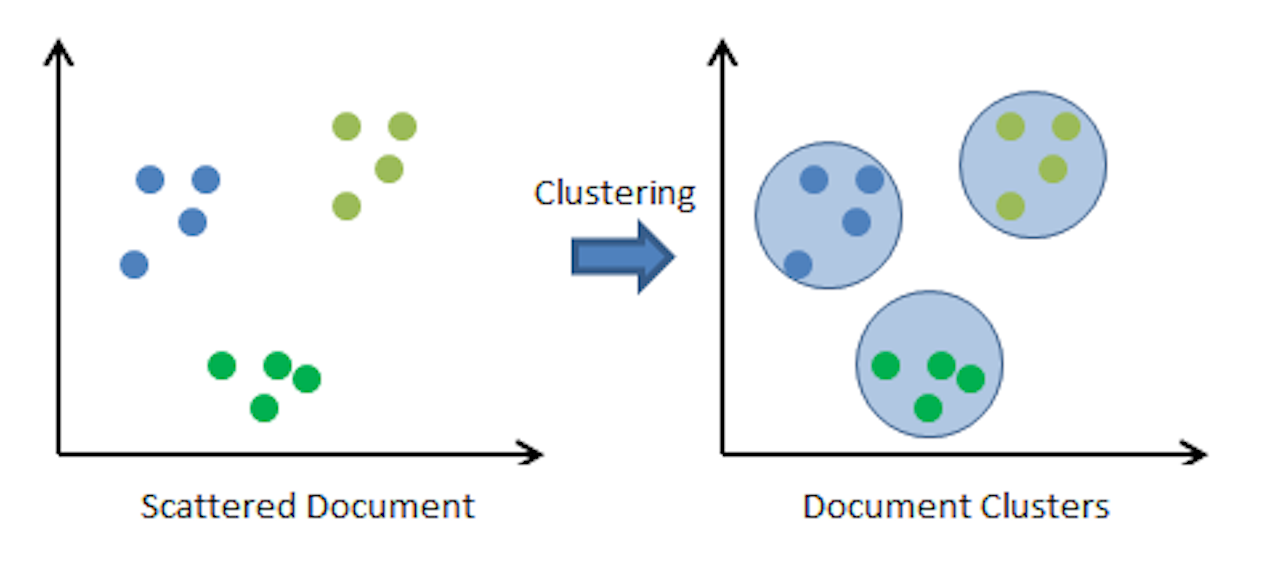
\includegraphics[width=\linewidth]{cluster}
\caption{example of clustering}
\label{fig:unsupervised-learning-scheme}
\end{figure}

%
% old
the software created is based on the paradigm of object-oriented programming. It
is a question of keeping the dependence on other libraries and frameworks to a
minimum, trying to guarantee the portability of the source code on platforms
with different hardware. The language chosen is C ++ with an intuitive use of
the Qt framework thus once again guaranteed portability, as well as the
graphical interface and high data performance the feature of compiled languages.
The software thus created inside presents the graphic structures of Qwidget, the
libraries to manage the Raspberry Pi camera seen in chapter 4 and the FLIR
Lepton SDK.

Once started, the application runs the main screen that can be divided into
three main areas: the preview section, the fusion section, the sidebar of the
commands. In the first section two widgets are shown that show the video streams
captured by the two cameras in separate threads, this thanks to the extensive
use of the ``\textbf{signal \& slot}"\footnote{Signals and slots are used for
communication between objects. The signals and slots mechanism is a central
feature of Qt and probably the part that differs most from the features provided
by other frameworks. Signals and slots are made possible by Qt's meta-object
system.\cite{qtsignalslot}} made available by Qt. In the sidebar of the
controls, there are the operations that allow you to change the color palette of
the thermal image, capture an image, select a particular blending method for the
two video streams and see them combined in the central section. The central
section, as anticipated, shows the superimposition of the thermal map on the RGB
image captured by the traditional photo camera.


